%
% File acl2015.tex
%
% Contact: car@ir.hit.edu.cn, gdzhou@suda.edu.cn
%%
%% Based on the style files for ACL-2014, which were, in turn,
%% Based on the style files for ACL-2013, which were, in turn,
%% Based on the style files for ACL-2012, which were, in turn,
%% based on the style files for ACL-2011, which were, in turn, 
%% based on the style files for ACL-2010, which were, in turn, 
%% based on the style files for ACL-IJCNLP-2009, which were, in turn,
%% based on the style files for EACL-2009 and IJCNLP-2008...

%% Based on the style files for EACL 2006 by 
%%e.agirre@ehu.es or Sergi.Balari@uab.es
%% and that of ACL 08 by Joakim Nivre and Noah Smith

\documentclass[11pt]{article}
\usepackage{acl2015}
\usepackage{times}
\usepackage{url}
\usepackage{latexsym}
\usepackage{graphicx}
\usepackage[style=numeric]{biblatex}

%\setlength\titlebox{5cm}

% You can expand the titlebox if you need extra space
% to show all the authors. Please do not make the titlebox
% smaller than 5cm (the original size); we will check this
% in the camera-ready version and ask you to change it back.


\title{Advances in Natural Language Processing with Deep Learning}

\author{Ruby Amyeen \\
  Institute for Computing in Research \\
  }

\begin{document}
\maketitle
\begin{abstract}
Natural Language Processing (NLP) is a branch of Artificial Intelligence (AI) that involves computers learning the natural language humans use to communicate- text and speech, and then using that knowledge to perform specific tasks. It is the intersection between linguistics, computer science, and machine learning. 
This study provides general landscaping of current NLP applications with a literary survey and how NLP models are implemented with neural networks. It also examines a single paper on automatic essay grading (AEG) and reproduces its results.


\end{abstract}

\section{Introduction}
The human language is filled with complexities such as grammar, syntax, sarcasm, and literary devices. Computers must be trained to understand these ambiguities to build effective NLP models that can perform text-generation and voice assistance tasks. The general process of NLP involves two main steps: data preprocessing and developing algorithms.

\subsection{Preprocessing}
In NLP, data preprocessing is a critical stage. The data in NLP models usually come in text and audio. Preprocessing includes tokenization, stop-word removal, and stemming and lemming. Once the data is cleaned, the next step is to convert it into numbers that are readable by a computer. Word embeddings are a common technique employed to turn words into vector representations and capture context and similarity between words. 
Figure 1 shows the word sky's three-dimensional embedding (vector representation) from https://projector.tensorflow.org/.

\begin{figure}
\centering
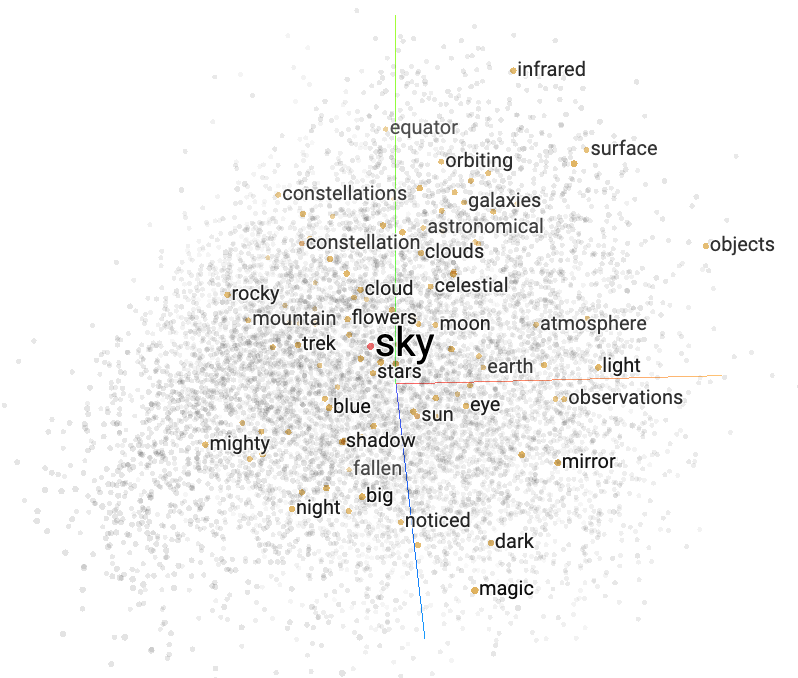
\includegraphics[width=0.3\textwidth]{sky_word_embedding.png}
\caption{3D embedding of the word sky}
\end{figure}

\subsection{Machine Learning}

Machine learning (ML) algorithms and NLP techniques allow computers to model, understand, and interpret human languages. There are two main machine learning types: supervised and unsupervised learning. Supervised learning is when a computer learns from correctly labeled inputs and can eventually predict the labels of unlabeled data points. The two subsets of supervised learning are regression and classification. Regression is when the model predicts a number from an infinite number of possible outputs, like the price of a house from the square foot area inputs. The model uses classification when it has to predict a class/category from a limited number of possible outputs—for example, determining if a cell is malignant or benign.
On the other hand, unsupervised learning is when none of the given data is labeled, and instead, the computer’s task is to find patterns in unlabeled data. Unsupervised learning includes clustering (grouping similar data points together), anomaly detection (finding unusual data points), and dimensionality reduction (compressing data using fewer numbers). While in the past, the developing algorithms aspect of NLP has been done through various ML approaches, including k-nearest neighbors, decision trees, and naïve Bayes, the field has been completely transformed and taken over by neural networks. 

\subsection{Neural Networks}
Neural networks mimic how neurons work and learn in the human brain. Figure 2 illustrates the x inputs in the input layer that are fed to the hidden layers with their weights and activation functions and then two possible output values in the output layer. The model learns to fit the data by changing its weights to minimize loss (the difference between the true output label and the predicted output label) using an optimization algorithm called gradient descent. 

\begin{figure}
\centering
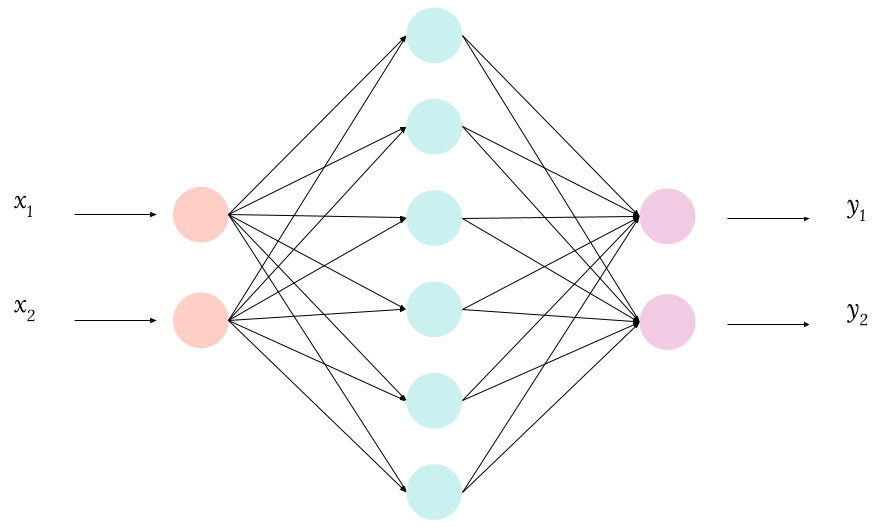
\includegraphics[width=0.4\textwidth]{nn.png}
\caption{Neural network with 2 inputs, 1 hidden layer, and 2 output values}
\end{figure}

%\begin{figure}
%\centering
%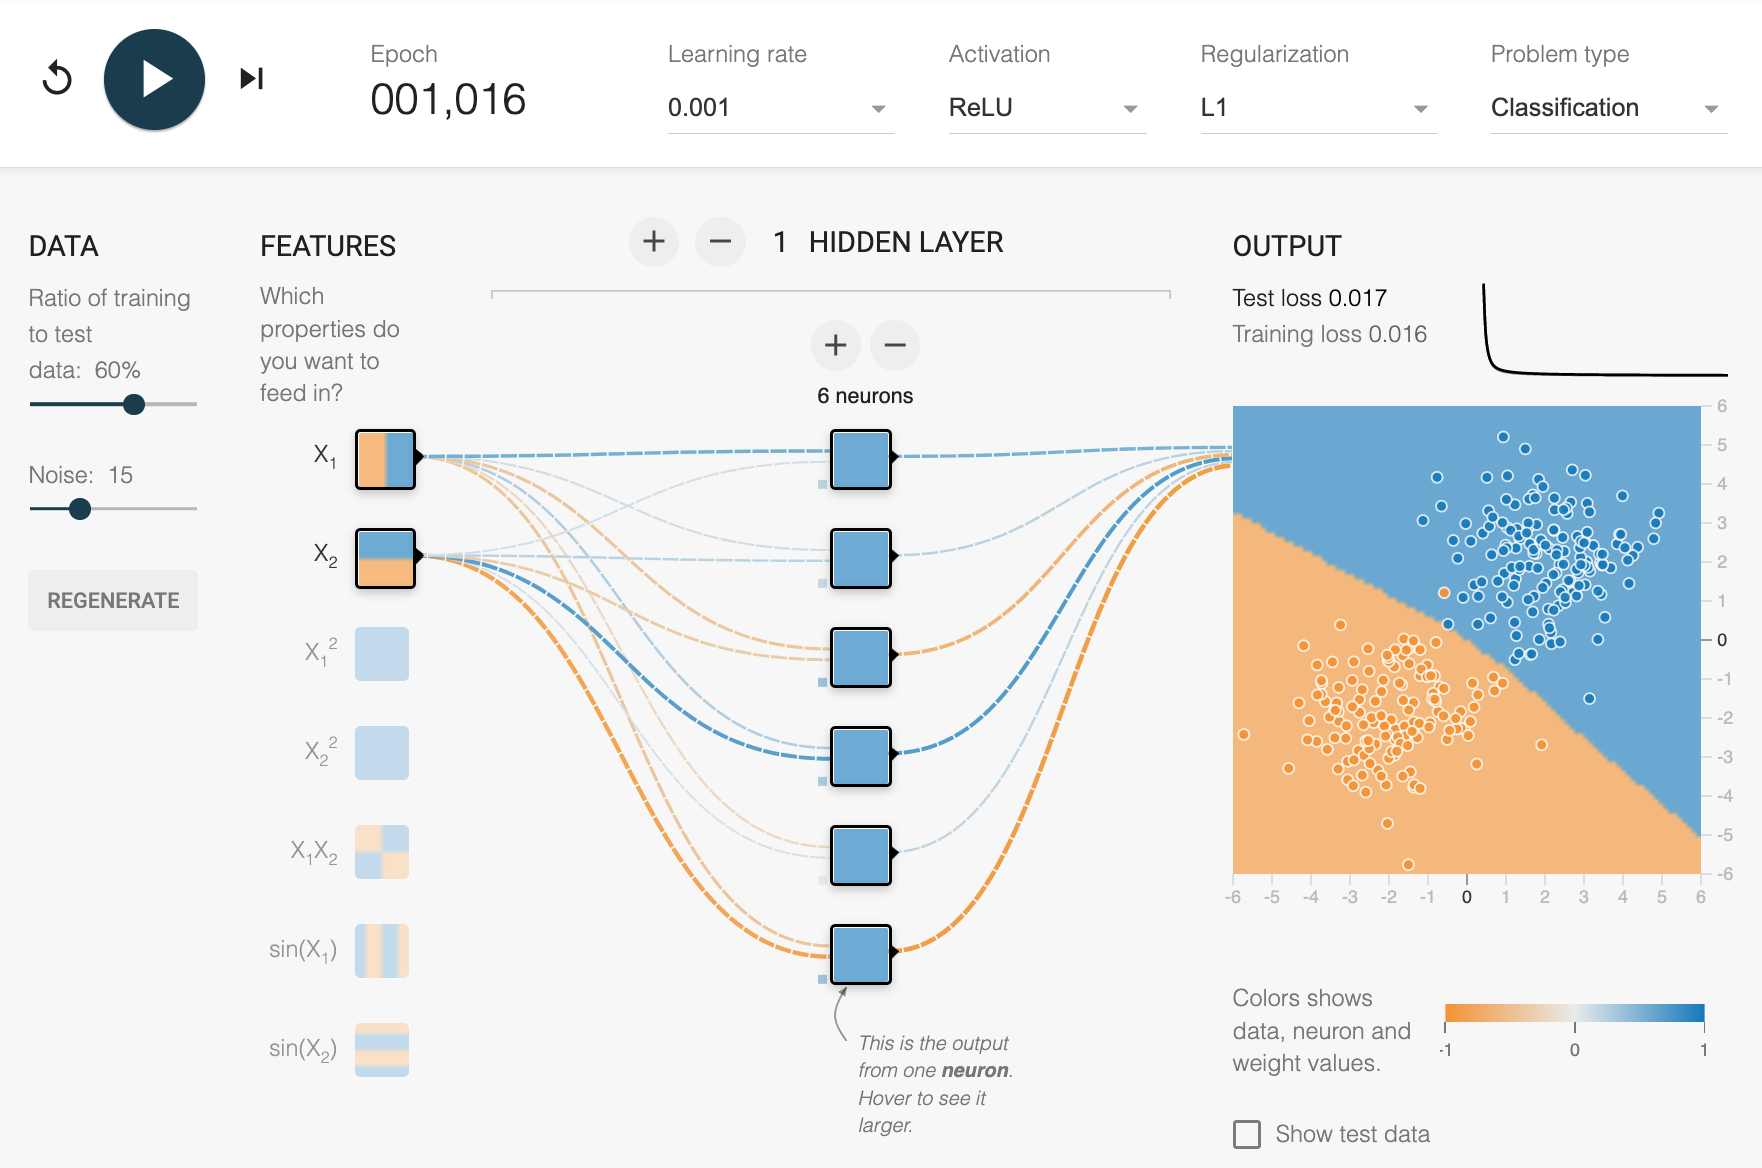
\includegraphics[width=0.4\textwidth]{demo.png}
%\caption{How the neural network learns as well as controlling hyper-parameters in a binary classification problem}
%\end{figure}


\subsubsection{Recurrent Neural Networks}
NLP typically uses Recurrent Neural Networks (RNNs) since they work well on sequential data (time series, text, audio, etc.). RNNs can represent context information because they keep information about past inputs for a long time (like humans but unlike traditional neural networks) with loops. This feature makes an RNN incredibly convenient for NLP when the learning problem is sequential. However, a challenge with RNNs is long-term dependency. Long-term dependency is when the true label output depends on an input far from the past. While RNNs cannot retain this information, Long Short Term Memory (LSTM) networks, a type of RNN, solve this problem and can learn long-term dependencies. Similarly, Gated Recurrent Units (GRU) can handle long-term dependencies while using less memory and performing faster than LSTMs, but perform worse than LSTMs on longer datasets.

\subsection{Transformers}

As mentioned before, long-term dependencies are a challenge for many neural networks. Transformers are a unique architecture that retains the relationships between all the words in a sentence. Transformers aren’t implemented with RNNs and only use attention mechanisms. They consist of an encoder and a decoder. An encoder extracts features from the input, and a decoder produces a prediction for the task using the features. BERT (Bi-directional Encoder Representation from Transformers) is a widely used pre-trained language model in deep neural networks. 


\section{NLP Applications - A Literary Survey}

\subsection{Methodology}
The NAACL is a widely recognized NLP annually held conference. To obtain a general landscape of NLP applications and the current state-of-the-art models, I conducted a literary survey with 20 papers from the 2022 NAACL conference under the heading “NLP Applications.” Since all of these papers are from 2022, they present recent findings and cover the latest developments in the field. 


\subsection{Findings}
This paper summarizes the findings that are relevant to NLP applications
\\[12pt]
\noindent
\textbf{Health}
\begin{itemize}
\item Bhanu Pratap Singh Rawat, Samuel Kovaly, Wilfred R. Pigeon, Hong Yu, \emph{ScAN: Suicide Attempt and Ideation Events Dataset}
\end{itemize}
Suicide is one of the leading causes of death, making it a primary public health concern. This study presents a neural network model that could lead to early intervention and suicide prevention—using a database of electronic health records (EHR). EHR includes a history of the patient’s suicide attempts (SA) and suicide ideations (SI) in the forms of admission notes, physician notes, and discharge summaries. The model can predict and monitor the patient’s suicide behaviors using the EHR database.

\begin{itemize}
\item Felix Drinkall, Stefan Zohren, Janet B. Pierrehumbert, \emph{Forecasting COVID-19 Caseloads Using Unsupervised Embedding Clusters of Social Media Posts}
\end{itemize}
With COVID-19 cases still rising, this study uses web search data to forecast the spread of infectious diseases. The model predicts COVID-19 caseloads by using Reddit post clusters. The advantage of this method is that Reddit posts are readily available and updated in real time. On the other hand, the disadvantages concern unequal access to the data depending on geographical location. The COVID-19 cases of some places are not recorded on Reddit or not uploaded regularly. 
\\[12pt]
\noindent
\textbf{Misinformation}
\begin{itemize}
\item Lin Tian, Xiuzhen Zhang, Jey Han Lau, \emph{DUCK: Rumour Detection on Social Media by Modelling User and Comment Propagation Networks}
\end{itemize}
Social media rumors are misinformation and can mislead the public, causing economic or social disruption. This research aims to stop the spread of misinformation. The model observes the user network (users who engage with the story) and the comment network (how users react to the story), then predicts the rumor with a true or false label.

\begin{itemize}
\item Fengzhu Zeng, Wei Gao, \emph{Early Rumor Detection Using Neural Hawkes Process with a New Benchmark Dataset}
\end{itemize}
This study aims to improve rumor detection applications. The scientists believe that combining early detection with general rumor detection leads to more accurate rumor detection. This model is more catered to early rumor detection.  

\begin{itemize}
\item Xuming Hu, Zhijiang Guo, Guanyu Wu, Aiwei Liu, Lijie Wen, Philip S. Yu, \emph{CHEF: A Pilot Chinese Dataset for Evidence-Based Fact-Checking}
\end{itemize}
Most rumor detection systems are in English. This study addresses the issue by combating misinformation in Chinese. It uses a Chinese dataset with 10,000 real-work claims and manually annotated evidence sentences and then predicts a true or false rumor label. A challenge researchers faced with this study was finding claims. They had to extract reliable evidence resulting in a lengthy process manually. Future work could address this concern. 

\begin{itemize}
\item Nan Hu, Zirui Wu, Yuxuan Lai, Xiao Liu, Yansong Feng, \emph{Dual-Channel Evidence Fusion for Fact Verification over Texts and Tables}
\end{itemize}
Typically fact extraction and verification tasks only use evidence in a single format. This paper uses both plain text and tables to capture the context in their original form. 
\\[12pt]
\noindent
\textbf{Politics}
\begin{itemize}
\item Wenqian Zhang, Shangbin Feng, Zilong Chen, Zhenyu Lei, Jundong Li, Minnan Luo, \emph{KCD: Knowledge Walks and Textual Cues Enhanced Political Perspective Detection in News Media}
\end{itemize}
Political perspective detection can help combat echo chambers, environments where the political leaning or a belief gets reinforced with repeated interactions with similar attitudes. This model aims to identify stances of text and then classify perspective labels (left wing or right wing). 

\begin{itemize}
\item Yibo Hu, Mohammad Saleh Hosseini, Erick Skorupa Parolin, Javier Osorio, Latifur Khan, Patrick T. Brandt, Vito J. D’Orazio, \emph{ConfliBERT: A Pre-trained Language Model for Political Conflict and Violence}
\end{itemize}
This paper addresses the challenge of analyzing conflict and political violence as it requires a lot of specific text to monitor the conflict. They have created a pre-trained model for political strife and violence available to the general public.  
\\[12pt]
\noindent
\textbf{Scoring/Error Detection}
\begin{itemize}
\item Muhammad Reza Qorib, Seung-Hoon Na, Hwee Tou Ng, \emph{Frustratingly Easy System Combination for Grammatical Error Correction}
\end{itemize}
This model takes a unique approach to detecting and correcting grammatical errors in the text. It extracts edits and classifies them as insertion, deletion, or substitution. Finally, it uses a generalized linear model to predict whether a modification should be kept or deleted. 

\begin{itemize}
\item Yongjie Wang, Chuan Wang, Ruobing Li, Hui Lin, \emph{On the Use of BERT for Automated Essay Scoring: Joint Learning of Multi-Scale Essay Representation}
\end{itemize}
Automated essay scoring (AES) would promote the development of automated assessment and reduce the burden of grading on teachers. This AES system accounts for multiple factors (word count, essay structure, vocabulary, syntactic complexity). It uses BERT, takes the preprocessed essay as the input, and outputs a score.

\begin{itemize}
\item Rahul Kumar, Sandeep Mathias, Sriparna Saha, Pushpak Bhattacharyya, \emph{Many Hands Make Light Work: Using Essay Traits to Automatically Score Essays}
\end{itemize}
Most research in automated essay grading (AEG) looks at essays holistically, often ignoring individual essay traits. This paper implements a multi-task learning approach (MTL) where the primary task is scoring the essay holistically, and auxiliary tasks score the essay traits. The results found that the MTL approach outperformed the STL model in accuracy and speed. 

\begin{itemize}
\item Rajat Agarwal, Varun Khurana, Karish Grover, Mukesh Mohania, Vikram Goyal, \emph{Multi-Relational Graph Transformer for Automatic Short Answer Grading}
\end{itemize}
Automatic Short Answer Grading (ASAG) hopes to alleviate the burden of grading. This model compares the correct answer with the student’s responses and gives the short answer a score. Currently, most methods compare the two answers without taking structural context into account; however, this approach proves to lower accuracy as structural context is vital for grading. 
\\[12pt]
\noindent
\textbf{Translation}
\begin{itemize}
\item Shanqing Cai, Subhashini Venugopalan, Katrin Tomanek, Ajit Narayanan, Meredith Ringel Morris, Michael P. Brenner, \emph{Context-Aware Abbreviation Expansion Using Large Language Models}
\end{itemize}
People with severely limited motor capabilities often communicate in abbreviations. This language model decodes the abbreviations from context. Context is critical in NLP because it helps determine the word's meaning and results in a more accurate model. 

\begin{itemize}
\item Zhewei Sun, Richard Zemel, Yang Xu, \emph{Semantically Informed Slang Interpretation}
\end{itemize}
Slang is a predominant informal language that’s hard for NLP models to interpret. While existing approaches use context, they disregard semantic extensions common in slang usage. This model uses both context and semantic appropriateness to analyze slang. Even in zero-shot and few-shot scenarios, this model performs well. This research is crucial to overcoming the obstacle of slang in NLP applications. 

\begin{itemize}
\item Shikhar Bharadwaj, Shirish Shevade, \emph{Efficient Constituency Tree based Encoding for Natural Language to Bash Translation}
\end{itemize}
Bash is a command line tool to manipulate files and directories efficiently. This model takes natural language text command and translates it to bash command, making computing more accessible to people with little command line knowledge.
\\[12pt]
\noindent
\textbf{Understanding Text Better}
\begin{itemize}
\item John S. Y. Lee, Ho Hung Lim, Carol Webster, \emph{Unsupervised Paraphrasability Prediction for Compound Nominalizations}
\end{itemize}
A nominalization is a noun created from verbs and adjectives. They are commonly found in academic and formal texts; however, they are hard to interpret because of the ambiguous semantic relation between the deverbal noun and its argument. Automated generation of paraphrasing clauses can help make the meanings more coherent. More specific NLP tasks can use this application if they require the interpretation of compound nominalizations to improve the accuracy of their models. 

\begin{itemize}
\item Naoki Otani, Michael Gamon, Sujay Kumar Jauhar, Mei Yang, Sri Raghu Malireddi, Oriana Riva, \emph{LITE: Intent-based Task Representation Learning Using Weak Supervision}
\end{itemize}
To-do lists are personal notes about things the user has to complete or remember. They tend to be short and under-specified, making it hard for current models to interpret them. This model implements a general encoding system that converts tasks into vector representations and can eventually lead to the development of task management tools from task prioritization to breaking down long-term tasks.
\\[12pt]
\noindent
\textbf{Semi-Supervised Learning}
\begin{itemize}
\item Hai-Ming Xu, Lingqiao Liu, Ehsan Abbasnejad, \emph{Progressive Class Semantic Matching for Semi-supervised Text Classification}
\end{itemize}
Annotation costs are high in text classification, which is required in many NLP applications. Most applications use supervised learning, which requires many expensive annotations. Semi-supervised learning is in the middle of supervised learning and unsupervised learning. It uses a small amount of labeled data and large amounts of unlabeled data, overcoming the high annotation costs. 
\\[12pt]
\noindent
\textbf{Finance}
\begin{itemize}
\item Ramit Sawhney, Shivam Agarwal, Vivek Mittal, Paolo Rosso, Vikram Nanda, Sudheer Chava, \emph{Cryptocurrency Bubble Detection: A New Stock Market Dataset, Financial Task and Hyperbolic Models}
\end{itemize}
Bubbles are irregular behavior of markets, often created by social media. Social media can heavily influence the stock market. To forecast bubbles, this model surveilled social media and the stock market.




\section{Code Replication}
I replicated the code from a paper presented at the 2021 NAACL conference: Sungho Jeon and Michael Strube, \emph{Countering the Influence of Essay Length in Neural Essay Scoring}. 

\subsection{Background}
Automated essay grading (AEG) is when a computer assigns a score for a given essay, trying to replicate human scoring results. After the release of the Kaggle Automated Student’s Assessment Prize (ASAP) Automatic Essay Grading (AEG) dataset, interest in this field has increased drastically. Jeon and Strube reveal that previous automated essay scoring systems cannot assess the quality of essays; instead, these models rely on essay length– a factor that is irrelevant to the quality of the essay. They found a high correlation between essay length and scores, which models exploited for top performance. Even if the model engineering didn’t specify the use of essay length, evidence shows that the correlation between length and score may still influence models. To test this theory, Jeon and Strube created a simple neural model that manipulated essay length and demonstrated that this model achieved performance comparable to the state-of-the-art neural models in the standard dataset. Since the Kaggle dataset had a very high correlation between essay length and score, Jeon and Strube also utilized the TOEFL dataset with a lower correlation to test if the model was effective without relying on essay length. This study proves that taking just essay content without essay length into account can improve the performance of AEG systems. 

\subsection{Dataset}
The dataset used was the ASAP dataset from Kaggle. It had a total of 8 essay sets with unique linguistic characteristics. Figure 3 shows the different prompts for each of the 8 essay sets. Some essay sets are persuasive/narrative, while others are source dependent. Each essay set has several essays written in response to the same essay prompt. There are 13,000 English essays written by American high school students from grades 7 to 10. In Figure 4, an example of an essay set is shown.


\begin{figure}
\centering
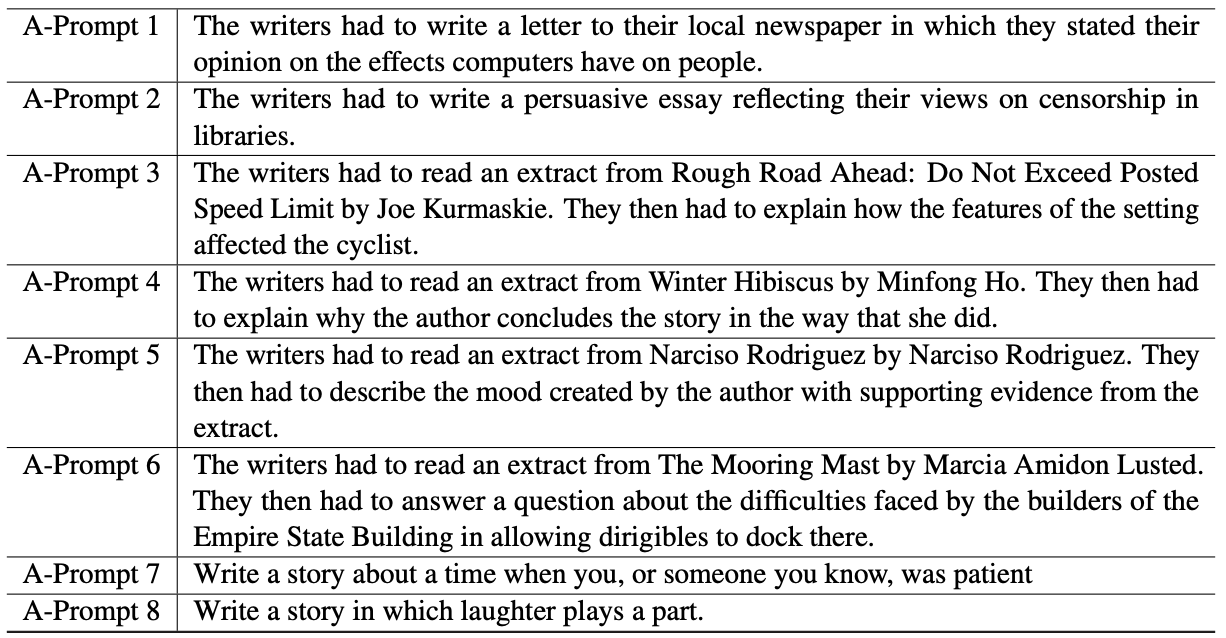
\includegraphics[width=0.4\textwidth]{prompts.png}
\caption{ASAP dataset prompts for the 8 essay sets}
\end{figure}

\begin{figure}
\centering
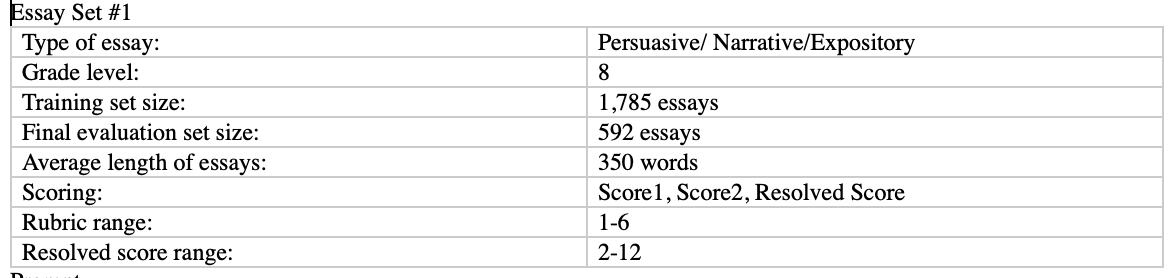
\includegraphics[width=0.4\textwidth]{essay_set.png}
\caption{Essay set \#1 from the ASAP dataset.}
\end{figure}

\subsection{Method}
To replicate the experiment, I used the sourced code from \url{https://github.com/sdeva14}.
After cloning the repository, I created a Conda environment to set up. Since the datasets were not included in the repository, I downloaded the dataset from Kaggle’s official website. I used the Kaggle dataset since it was publicly available, unlike the TOEFL dataset. I downloaded the pre-trained word embeddings to evaluate the ilcr-kld model, which considered essay content with KL-divergence by comparing word distribution with an input essay and essays with different scores. The data was split into five folds into the .txt files located in \url{https://github.com/nusnlp/nea}. Since the laptop I used to reproduce the experiments did not have a GPU, I had to change the commands in the build\_config.py file to configure for CPU instead of GPU. Furthermore, I modified code lines for the python3 version and did some extra debugging. 

\section{Results}
I was able to reproduce the results from the paper. The ilcr-kld model performed almost as well as state-of-the-art models on the ASAP dataset. Figures 5 and 6 show the results printed onto the console for fold 1 with Quadratic Weighted Kappa (QWK) scoring. QWK is an evaluation metric based on the confusion metric. QWK rewards match and punish mismatches better than Linear Weighted Kappa. 

\begin{figure}
\centering
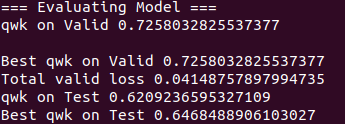
\includegraphics[width=0.4\textwidth]{results1.png}
\caption{Evaluating the model with QWK}
\end{figure}


\begin{figure}
\centering
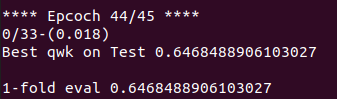
\includegraphics[width=0.4\textwidth]{resultstest.png}
\caption{Best QWK test set score for fold 1}
\end{figure}

\section{Conclusion and Future Work}
\subsection{Review}
Deep learning has completely transformed the field of NLP applications. Throughout this project, I learned about the different types of neural networks involved in NLP applications and reviewed all the NLP application papers presented at the NAACL 2022 conference. 

\subsection{Automated Essay Grading (AEG)}
This study encourages future work to examine a dataset's natural characteristics and whether it skews the learning or considers irrelevant factors to the model's assessment. For future work, the next step would be to improve the model and evaluate it against the baseline model. In the area of AEG, a model could take the type of essay into account (argumentative, narrative, informative) because of style changes between essay types. Would the model achieve high performance on all the different types of essays? Furthermore, it would be helpful if the model could provide text feedback for what the writer could improve on, just like a human scorer. One concern in this field is overfitting a particular dataset– like how the state-of-the-art models performed better on the ASAP dataset than the TOEFL dataset.



\section*{Acknowledgments}
Thank you Ameeta Agrawal for mentoring me throughout this project. I would also like to thank the Institute for Computing in Research for providing this research opportunity. 


% include your own bib file like this:
%\bibliographystyle{acl}
%\bibliography{acl2015}

\begin{thebibliography}{50}

\bibitem{}
Bhanu Pratap Singh Rawat, Samuel Kovaly, Hong Yu, and Wilfred Pigeon. 2022. ScAN: Suicide Attempt and Ideation Events Dataset. In \emph{Proceedings of the 2022 Conference of the North American Chapter of the Association for Computational Linguistics: Human Language Technologies}, pages 1029–1040, Seattle, United States. Association for Computational Linguistics.

\bibitem{}
Felix Drinkall, Stefan Zohren, and Janet Pierrehumbert. 2022. Forecasting COVID-19 Caseloads Using Unsupervised Embedding Clusters of Social Media Posts. In \emph{Proceedings of the 2022 Conference of the North American Chapter of the Association for Computational Linguistics: Human Language Technologies}, pages 1471–1484, Seattle, United States. Association for Computational Linguistics.

\bibitem{}
Fengzhu Zeng and Wei Gao. 2022. Early Rumor Detection Using Neural Hawkes Process with a New Benchmark Dataset. In \emph{Proceedings of the 2022 Conference of the North American Chapter of the Association for Computational Linguistics: Human Language Technologies}, pages 4105–4117, Seattle, United States. Association for Computational Linguistics.

\bibitem{}
Haiming Xu, Lingqiao Liu, and Ehsan Abbasnejad. 2022. Progressive Class Semantic Matching for Semi-supervised Text Classification. In \emph{Proceedings of the 2022 Conference of the North American Chapter of the Association for Computational Linguistics: Human Language Technologies}, pages 3003–3013, Seattle, United States. Association for Computational Linguistics.

\bibitem{}
John Sie Yuen Lee, Ho Hung Lim, and Carol Carol Webster. 2022. Unsupervised Paraphrasability Prediction for Compound Nominalizations. In \emph{Proceedings of the 2022 Conference of the North American Chapter of the Association for Computational Linguistics: Human Language Technologies}, pages 3254–3263, Seattle, United States. Association for Computational Linguistics.

\bibitem{}
Jonathan Rusert and Padmini Srinivasan. 2022. Don’t sweat the small stuff, classify the rest: Sample Shielding to protect text classifiers against adversarial attacks. In \emph{Proceedings of the 2022 Conference of the North American Chapter of the Association for Computational Linguistics: Human Language Technologies}, pages 2716–2725, Seattle, United States. Association for Computational Linguistics.

\bibitem{}
Kaveh Taghipour and Hwee Tou Ng. 2016. A Neural Approach to Automated Essay Scoring. In \emph{Proceedings of the 2016 Conference on Empirical Methods in Natural Language Processing}, pages 1882–1891, Austin, Texas. Association for Computational Linguistics.

\bibitem{}
Khurana, D., Koli, A., Khatter, K. \emph{et al.} Natural language processing: state of the art, current trends and challenges. \emph{Multimed Tools Appl} (2022). https://doi.org/10.1007/s11042-022-13428-4


\bibitem{}
Lin Tian, Xiuzhen Zhang, and Jey Han Lau. 2022. DUCK: Rumour Detection on Social Media by Modelling User and Comment Propagation Networks. In \emph{Proceedings of the 2022 Conference of the North American Chapter of the Association for Computational Linguistics: Human Language Technologies}, pages 4939–4949, Seattle, United States. Association for Computational Linguistics.

\bibitem{}
Muhammad Qorib, Seung-Hoon Na, and Hwee Tou Ng. 2022. Frustratingly Easy System Combination for Grammatical Error Correction. In \emph{Proceedings of the 2022 Conference of the North American Chapter of the Association for Computational Linguistics: Human Language Technologies}, pages 1964–1974, Seattle, United States. Association for Computational Linguistics.

\bibitem{}
Nan Hu, Zirui Wu, Yuxuan Lai, Xiao Liu, and Yansong Feng. 2022. Dual-Channel Evidence Fusion for Fact Verification over Texts and Tables. In \emph{Proceedings of the 2022 Conference of the North American Chapter of the Association for Computational Linguistics: Human Language Technologies}, pages 5232–5242, Seattle, United States. Association for Computational Linguistics.

\bibitem{}
Naoki Otani, Michael Gamon, Sujay Kumar Jauhar, Mei Yang, Sri Raghu Malireddi, and Oriana Riva. 2022. LITE: Intent-based Task Representation Learning Using Weak Supervision. In \emph{Proceedings of the 2022 Conference of the North American Chapter of the Association for Computational Linguistics: Human Language Technologies}, pages 2410–2424, Seattle, United States. Association for Computational Linguistics.

\bibitem{}
Rahul Kumar, Sandeep Mathias, Sriparna Saha, and Pushpak Bhattacharyya. 2022. Many Hands Make Light Work: Using Essay Traits to Automatically Score Essays. In \emph{Proceedings of the 2022 Conference of the North American Chapter of the Association for Computational Linguistics: Human Language Technologies}, pages 1485–1495, Seattle, United States. Association for Computational Linguistics.

\bibitem{}
Rajat Agarwal, Varun Khurana, Karish Grover, Mukesh Mohania, and Vikram Goyal. 2022. Multi-Relational Graph Transformer for Automatic Short Answer Grading. In \emph{Proceedings of the 2022 Conference of the North American Chapter of the Association for Computational Linguistics: Human Language Technologies}, pages 2001–2012, Seattle, United States. Association for Computational Linguistics.

\bibitem{}
Ramit Sawhney, Shivam Agarwal, Vivek Mittal, Paolo Rosso, Vikram Nanda, and Sudheer Chava. 2022. Cryptocurrency Bubble Detection: A New Stock Market Dataset, Financial Task \& Hyperbolic Models. In \emph{Proceedings of the 2022 Conference of the North American Chapter of the Association for Computational Linguistics: Human Language Technologies}, pages 5531–5545, Seattle, United States. Association for Computational Linguistics.

\bibitem{}
Shanqing Cai, Subhashini Venugopalan, Katrin Tomanek, Ajit Narayanan, Meredith Morris, and Michael Brenner. 2022. Context-Aware Abbreviation Expansion Using Large Language Models. In \emph{Proceedings of the 2022 Conference of the North American Chapter of the Association for Computational Linguistics: Human Language Technologies}, pages 1261–1275, Seattle, United States. Association for Computational Linguistics.

\bibitem{}
Shikhar Bharadwaj and Shirish Shevade. 2022. Efficient Constituency Tree based Encoding for Natural Language to Bash Translation. In \emph{Proceedings of the 2022 Conference of the North American Chapter of the Association for Computational Linguistics: Human Language Technologies}, pages 3159–3168, Seattle, United States. Association for Computational Linguistics.

\bibitem{}
Sungho Jeon and Michael Strube. 2021. Countering the Influence of Essay Length in Neural Essay Scoring. In \emph{Proceedings of the Second Workshop on Simple and Efficient Natural Language Processing}, pages 32–38, Virtual. Association for Computational Linguistics.

\bibitem{}
Wenqian Zhang, Shangbin Feng, Zilong Chen, Zhenyu Lei, Jundong Li, and Minnan Luo. 2022. KCD: Knowledge Walks and Textual Cues Enhanced Political Perspective Detection in News Media. In \emph{Proceedings of the 2022 Conference of the North American Chapter of the Association for Computational Linguistics: Human Language Technologies}, pages 4129–4140, Seattle, United States. Association for Computational Linguistics.

\bibitem{}
Xuming Hu, Zhijiang Guo, GuanYu Wu, Aiwei Liu, Lijie Wen, and Philip Yu. 2022. CHEF: A Pilot Chinese Dataset for Evidence-Based Fact-Checking. In \emph{Proceedings of the 2022 Conference of the North American Chapter of the Association for Computational Linguistics: Human Language Technologies}, pages 3362–3376, Seattle, United States. Association for Computational Linguistics.

\bibitem{}
Yibo Hu, MohammadSaleh Hosseini, Erick Skorupa Parolin, Javier Osorio, Latifur Khan, Patrick Brandt, and Vito D’Orazio. 2022. ConfliBERT: A Pre-trained Language Model for Political Conflict and Violence. In \emph{Proceedings of the 2022 Conference of the North American Chapter of the Association for Computational Linguistics: Human Language Technologies}, pages 5469–5482, Seattle, United States. Association for Computational Linguistics.

\bibitem{}
Yongjie Wang, Chuang Wang, Ruobing Li, and Hui Lin. 2022. On the Use of Bert for Automated Essay Scoring: Joint Learning of Multi-Scale Essay Representation. In \emph{Proceedings of the 2022 Conference of the North American Chapter of the Association for Computational Linguistics: Human Language Technologies}, pages 3416–3425, Seattle, United States. Association for Computational Linguistics.

\bibitem{}
Yoonseok Yang, Kyu Seok Kim, Minsam Kim, and Juneyoung Park. 2022. GRAM: Fast Fine-tuning of Pre-trained Language Models for Content-based Collaborative Filtering. In \emph{Proceedings of the 2022 Conference of the North American Chapter of the Association for Computational Linguistics: Human Language Technologies}, pages 839–851, Seattle, United States. Association for Computational Linguistics.

\bibitem{}
Zhewei Sun, Richard Zemel, and Yang Xu. 2022. Semantically Informed Slang Interpretation. In \emph{Proceedings of the 2022 Conference of the North American Chapter of the Association for Computational Linguistics: Human Language Technologies}, pages 5213–5231, Seattle, United States. Association for Computational Linguistics.






\end{thebibliography}

\end{document}